\documentclass[12pt]{article}

\usepackage{packages/sbc/sbc-template}
\usepackage{graphicx,url}
\usepackage[utf8]{inputenc}
\usepackage[english]{babel}


\sloppy

\title{Code retrieval task analysis}

\author{Henrique Krausbug Correa\inst{1}, Viviane Pereira Moreira\inst{1}, Dennis Giovani Balreira\inst{1}}


\address{Instituto de Informática -- Universidade Federal do Rio Grande do Sul
  (UFRGS)\\
  Caixa Postal 15.064 -- 91.501-970 -- Porto Alegre -- RS -- Brazil
  \email{\{henrique,viviane,dgbalreira\}@inf.ufrgs.br}
}

\begin{document} 

\maketitle


% ( 150 words approximately )
\begin{abstract}
  TODO
\end{abstract}
     
% \begin{resumo} 
%   TODO
% \end{resumo}

\section{Introduction}
% (1 page)

% Context: Why is code retrieval important in NLP? What is XCodeEval’s role?

% Motivation:
%  - XCodeEval NL-Code task benchmark reports a great accuracy for all languages, but D language has a lower accuracy.
%  - Authors statement: "We suspect that the limited availability of resources for D in both The Stack (Kocetkov et al., 2022) dataset (training corpora of StarEncoder) and our XCODEEVAL dataset could account for this discrepancy. Also, the presence of more hard negative candidates (i.e., very similar to a correct code) makes it a challenging task to identify similar codes."
%  - However, by checking TABLE 4, D dataset size is greater than other languages such as Perl and Ocaml, which have higher accuracy. 

% Research questions:
%   - What is the root cause analysis for D language lower accuracy on code retrieval tasks?
%   - Can this performance be improved based on NLP class topics and published articles related to this topic?

Modern software development increasingly relies on AI-powered tools that combine code retrieval and generation capabilities to assist developers.
Recent systems like RepoCoder \cite{Zhang2023} demonstrate how iterative retrieval-generation pipelines can leverage repository-wide context for code completion.
This highlights the importance of precise code retrieval as a foundation for AI-assisted programming tools — from IDE autocompletion to documentation generation and code reuse recommendation systems \cite{Ziegler2022}.
However, to be effective, code retrieval systems must address two primary challenges:

\begin{itemize}
  \item \textbf{Semantic-Execution Gap}: Bridging the disparity between natural language intent (queries) and executable implementations (retrieval targets), requiring understanding of both functionality and syntax \cite{Wan2019}
  \item \textbf{Multilingual Context}: As shown in repository-level tools like RepoCoder, retrieval must handle cross-file dependencies and language-specific patterns while maintaining execution correctness
\end{itemize}

The XCodeEval benchmark \cite{Khan2023} formalizes these requirements through its NL-Code retrieval task over 25M coding examples from about 7.5K unique algorithmic problems. These tasks evaluate systems on their ability to match natural language problem descriptions with executable implementations across 17 programming languages. For evaluation and analysis, it uses the StarEncoder \cite{Li2023} architecture and computed the top-k retrieval accuracy for each of the 17 query languages. Table \ref{tab:xcodeeval-performance} summarizes the performance of StarEncoder on the XCodeEval benchmark for a subset of languages. Author's discussion of results is as follows:

\begin{quote}
\textit{``For NL-Code, performance is good across all languages except for D. We suspect that the limited availability of resources for D in both The Stack \cite{Kocetkov2022} dataset (training corpora of StarEncoder) and our XCodeEval dataset could account for this discrepancy. Also, the presence of more hard negative candidates (i.e., very similar to a correct code) makes it a challenging task to identify similar codes.''}~\cite{Khan2023}
\end{quote}

\begin{table}[ht]
\centering
\caption{Summary of performance of StarEncoder \cite{Li2023}
for k = 100 in ~\cite{Khan2023}}
\label{tab:xcodeeval-performance}
\begin{tabular}{lccccccc}
\hline
\textbf{Metric} & \textbf{C++} & \textbf{Java} & \textbf{Python} & \textbf{D} & \textbf{Perl} & \textbf{Ocaml} & \textbf{AVG.} \\
\hline
Acc@K & 83.81 & 84.72 & 84.57 & 68.98 & 81.33 & 85.45 & 83.83 \\
\hline
\end{tabular}
\end{table}

However, our analysis reveals a notable performance discrepancy in the XCodeEval benchmark: while the average top-100 retrieval accuracy across languages is 83.83\%, the D programming language achieves only 68.98\%. This is surprising given the data distribution shown in Table~\ref{tab:xcodeeval-selected}, which presents the three languages with the largest and smallest retrieval corpus sizes.

As shown, D has a larger training set and a greater corpus size than some better-performing languages such as Perl and Ocaml. In contrast, languages like C++ and Java have much larger corpora, yet D's retrieval accuracy is significantly lower than even languages with smaller datasets.

This contradicts the common assumption that dataset or corpus size is the primary determinant of retrieval performance. Instead, as echoed in repository-level studies~\cite{Zhang2023}, retrieval quality appears to depend more on the context relevance and characteristics of the data than on its quantity. This motivates a deeper investigation into the factors affecting D's performance.

\begin{table}[ht]
\centering
\caption{Retrieval statistics for selected languages in ~\cite{Khan2023}}
\label{tab:xcodeeval-selected}
\begin{tabular}{lrrr}
\hline
\textbf{Language} & \textbf{Train Size} & \textbf{Test Size} & \textbf{Corpus Size} \\
\hline
C++     & 6,181  & 1,098   & 18,212,508 \\
Java    & 5,930  & 1,021   & 2,523,044 \\
Python  & 4,930  & 859     & 2,290,854 \\
D       & 3,359  & 521     & 15,984 \\
Perl    & 1,276  & 412     & 11,035 \\
Ocaml   & 1,424  & 381     & 7,012 \\
\hline
\end{tabular}
\end{table}

We investigate:
\begin{itemize}
    \item What factors beyond dataset size contribute to D's lower retrieval performance?
    % \item How does the quality and characteristics of "hard negatives" differ for D compared to other languages?
    \item Is it possible to improve retrieval accuracy for low-resource languages through targeted NLP approaches?
\end{itemize}

This work aims to:
\begin{enumerate}
    \item Reproduce the XCodeEval NL-Code retrieval benchmark using the specified Dense Passage Retrieval (DPR) architecture with StarEncoder \cite{Li2023}
    % \item Conduct a thorough analysis of the D language performance anomaly
    \item Investigate whether standard NLP techniques for low-resource scenarios can improve results
\end{enumerate}

The remainder of this paper is structured as follows:
Section 2 covers background on code retrieval and the XCodeEval benchmark.
Section 3 reviews related work.
Section 4 details our methodology for benchmark reproduction.
Section 5 presents experimental results, and
Section 6 concludes with findings and future directions.

\section{Background}

% (1–2 pages)

% Terminilogy: Define key terms (e.g., code retrieval, dense passage retrieval).

% XCodeEval Benchmark: Tasks, dataset structure, and original paper’s setup.

% Dense Passage Retrieval (DPR): How it works, why it’s used for code retrieval.

XCodeEval Benchmark

The XCodeEval benchmark is designed to evaluate neural retrieval models in the context of programming tasks. It contains:

    A training dataset, comprising (query, positive code, negative code) triplets (Figure~\ref{fig:training}).


\begin{figure}[ht]
\centering
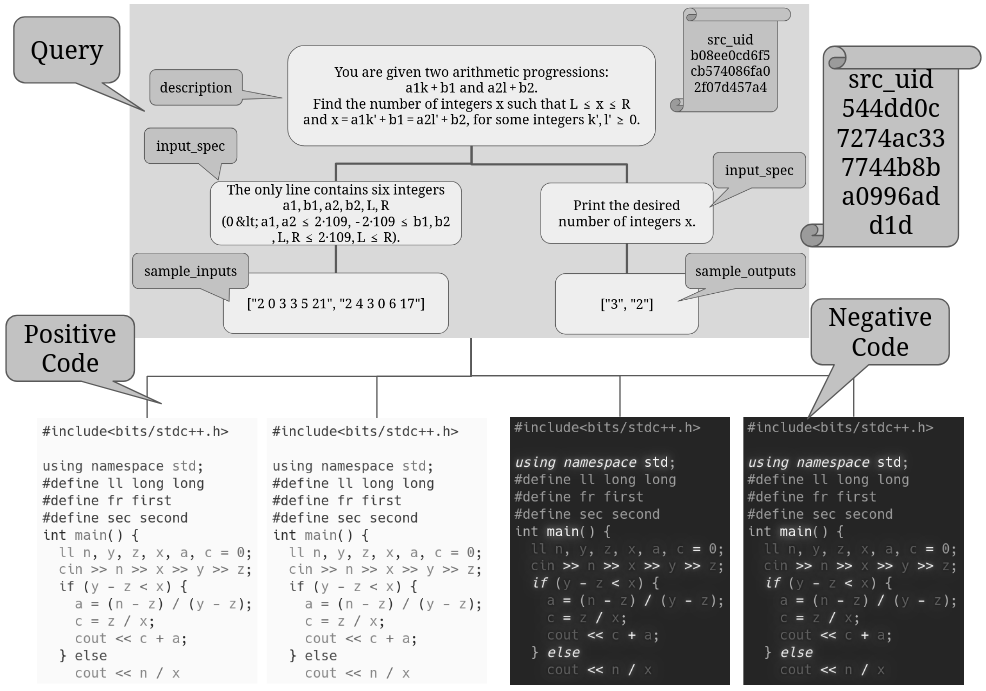
\includegraphics[width=1.0\textwidth]{images/task-gray.png}
\caption{Training dataset sample with query, positive and negative code}
\label{fig:training}
\end{figure}


\section{Related Work}

% (1–2 pages)

% Post Work: Summarize key papers on code retrieval that cite XCodeEval and criticize its limitations.

\section{Methodology}

%  (2–3 pages)

% Describe your approach to reproducing the XCodeEval benchmark.

% Data Preparation: How you processed XCodeEval (NL-Code template, corpus format).

% Model Setup:

%   DPR architecture (query/corpus encoders, multilingual training).

%   Hyperparameter (batch size, seq length, epochs) from the original paper.

% Evaluation Plan: Top-*k* accuracy (*k*=100), corpus/query embedding generation.

\section{Experimental Results}

% (3–4 pages)

% Describe framework, tools retrieval task results, and any preliminary findings.

% Expected vs. Actual: Compare original paper’s metrics to your observations.

% Possible Reasons for Divergence:

%   Training time insufficient? Hyperparameters not optimized?

%   Data preprocessing differences (e.g., template formatting).

% Qualitative Examples: Show some query-corpus pairs (even if not evaluated fully).

\section{Conclusion}

% (0.5 page)

% Lessons Learned: What would you do differently with more time/resources?

% Summary of efforts, challenges, and open questions.

% Alternative Approaches: Smaller models (e.g., ColBERT), approximate nearest-neighbor search (FAISS).

% Broader Implications: Reproducibility challenges in NLP research.

\bibliographystyle{packages/sbc/sbc}
\bibliography{paper}

\end{document}
